\documentclass[11pt]{beamer}
\usetheme{Warsaw}
\usepackage[utf8]{inputenc}
\usepackage{natbib}
\usepackage{amsmath}
\usepackage{graphicx}
\usepackage{subcaption}
\usepackage{tikz}
\usepackage{hyperref}
\setbeamertemplate{footline}[frame number]

\hypersetup{
    colorlinks=true,
    linkcolor=white,
    filecolor=magenta,      
    urlcolor=blue,
}


\title{Projet PSTALN}
\subtitle{Prédiction des \textit{morphy}}
\author{Cléa Han, Yanis Labeyrie et Adrien Zabban}
\date{15 janvier 2024}

\begin{document}

\maketitle

\begin{frame}{Le but: prédire les \textit{morphy}}
    \begin{figure}[b]
        \centering
        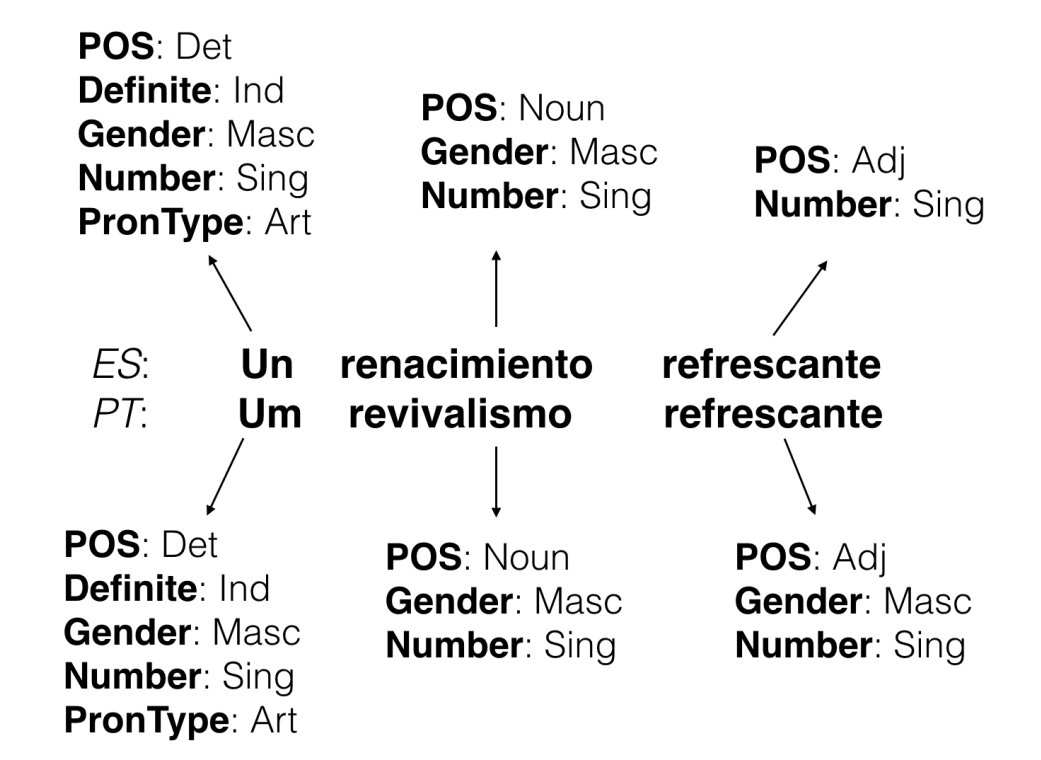
\includegraphics[width=0.8\textwidth]{morphy.png}
        % 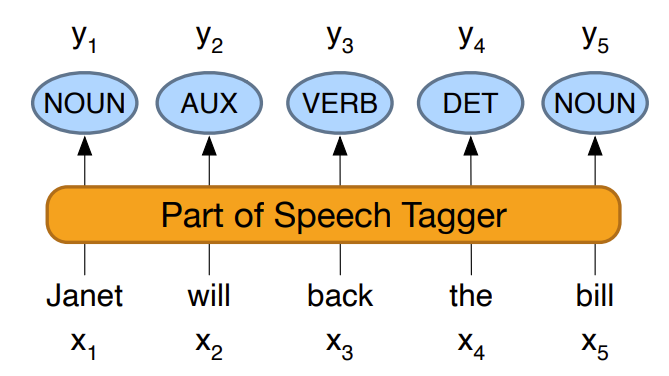
\includegraphics[width=0.40\textwidth]{pos.png}
        \caption{Tag morphologique d'une phrase portugaise et sa traduction en espagnol.}
    \end{figure}
\end{frame}

\begin{frame}{Les Données: Le dataset}
    Nous avons utilisé le dataset Universal Dependencies 2.13.

    Le dataset en français contient:
    \begin{itemize}
        \item 47498 phrases
        \item 849476 mots
        \item 76048 mots uniques
    \end{itemize}

    On a recensé:
    \begin{itemize}
        \item 19 classes \textit{pos}.
        \item 28 classes \textit{morphy}, dont le nombre maximun de possibilités est 13.
    \end{itemize}
\end{frame}

\begin{frame}{Les Données: Le padding}

\end{frame}

\begin{frame}{Les Données: La gestion des mots inconnus}

\end{frame}

\begin{frame}{Les Données: Encodage des labels}

\end{frame}

\begin{frame}{Modèle \textit{GET\_POS}}
    \begin{figure}
        \centering
        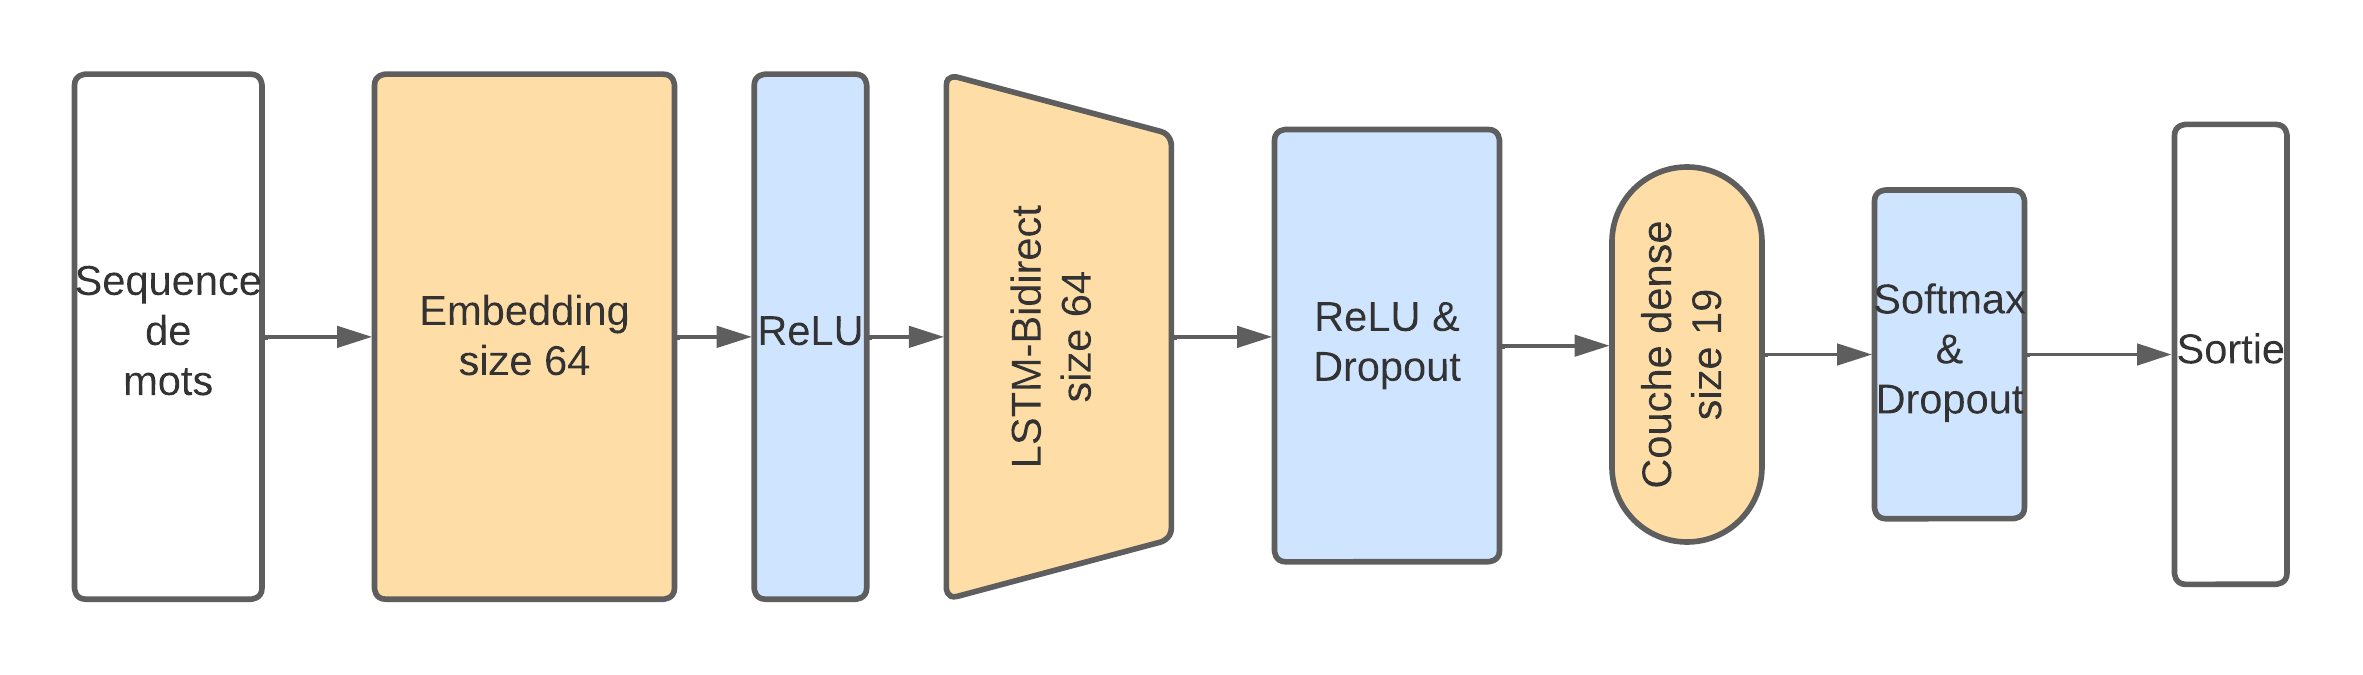
\includegraphics[width=\textwidth]{get_pos.png}
        \caption{Modèle \textit{GET\_POS}}
        \label{fig: model getpos}
    \end{figure} 
\end{frame}

\begin{frame}{Modèle \textit{SUPERTAG}}
    \begin{figure}
        \centering
        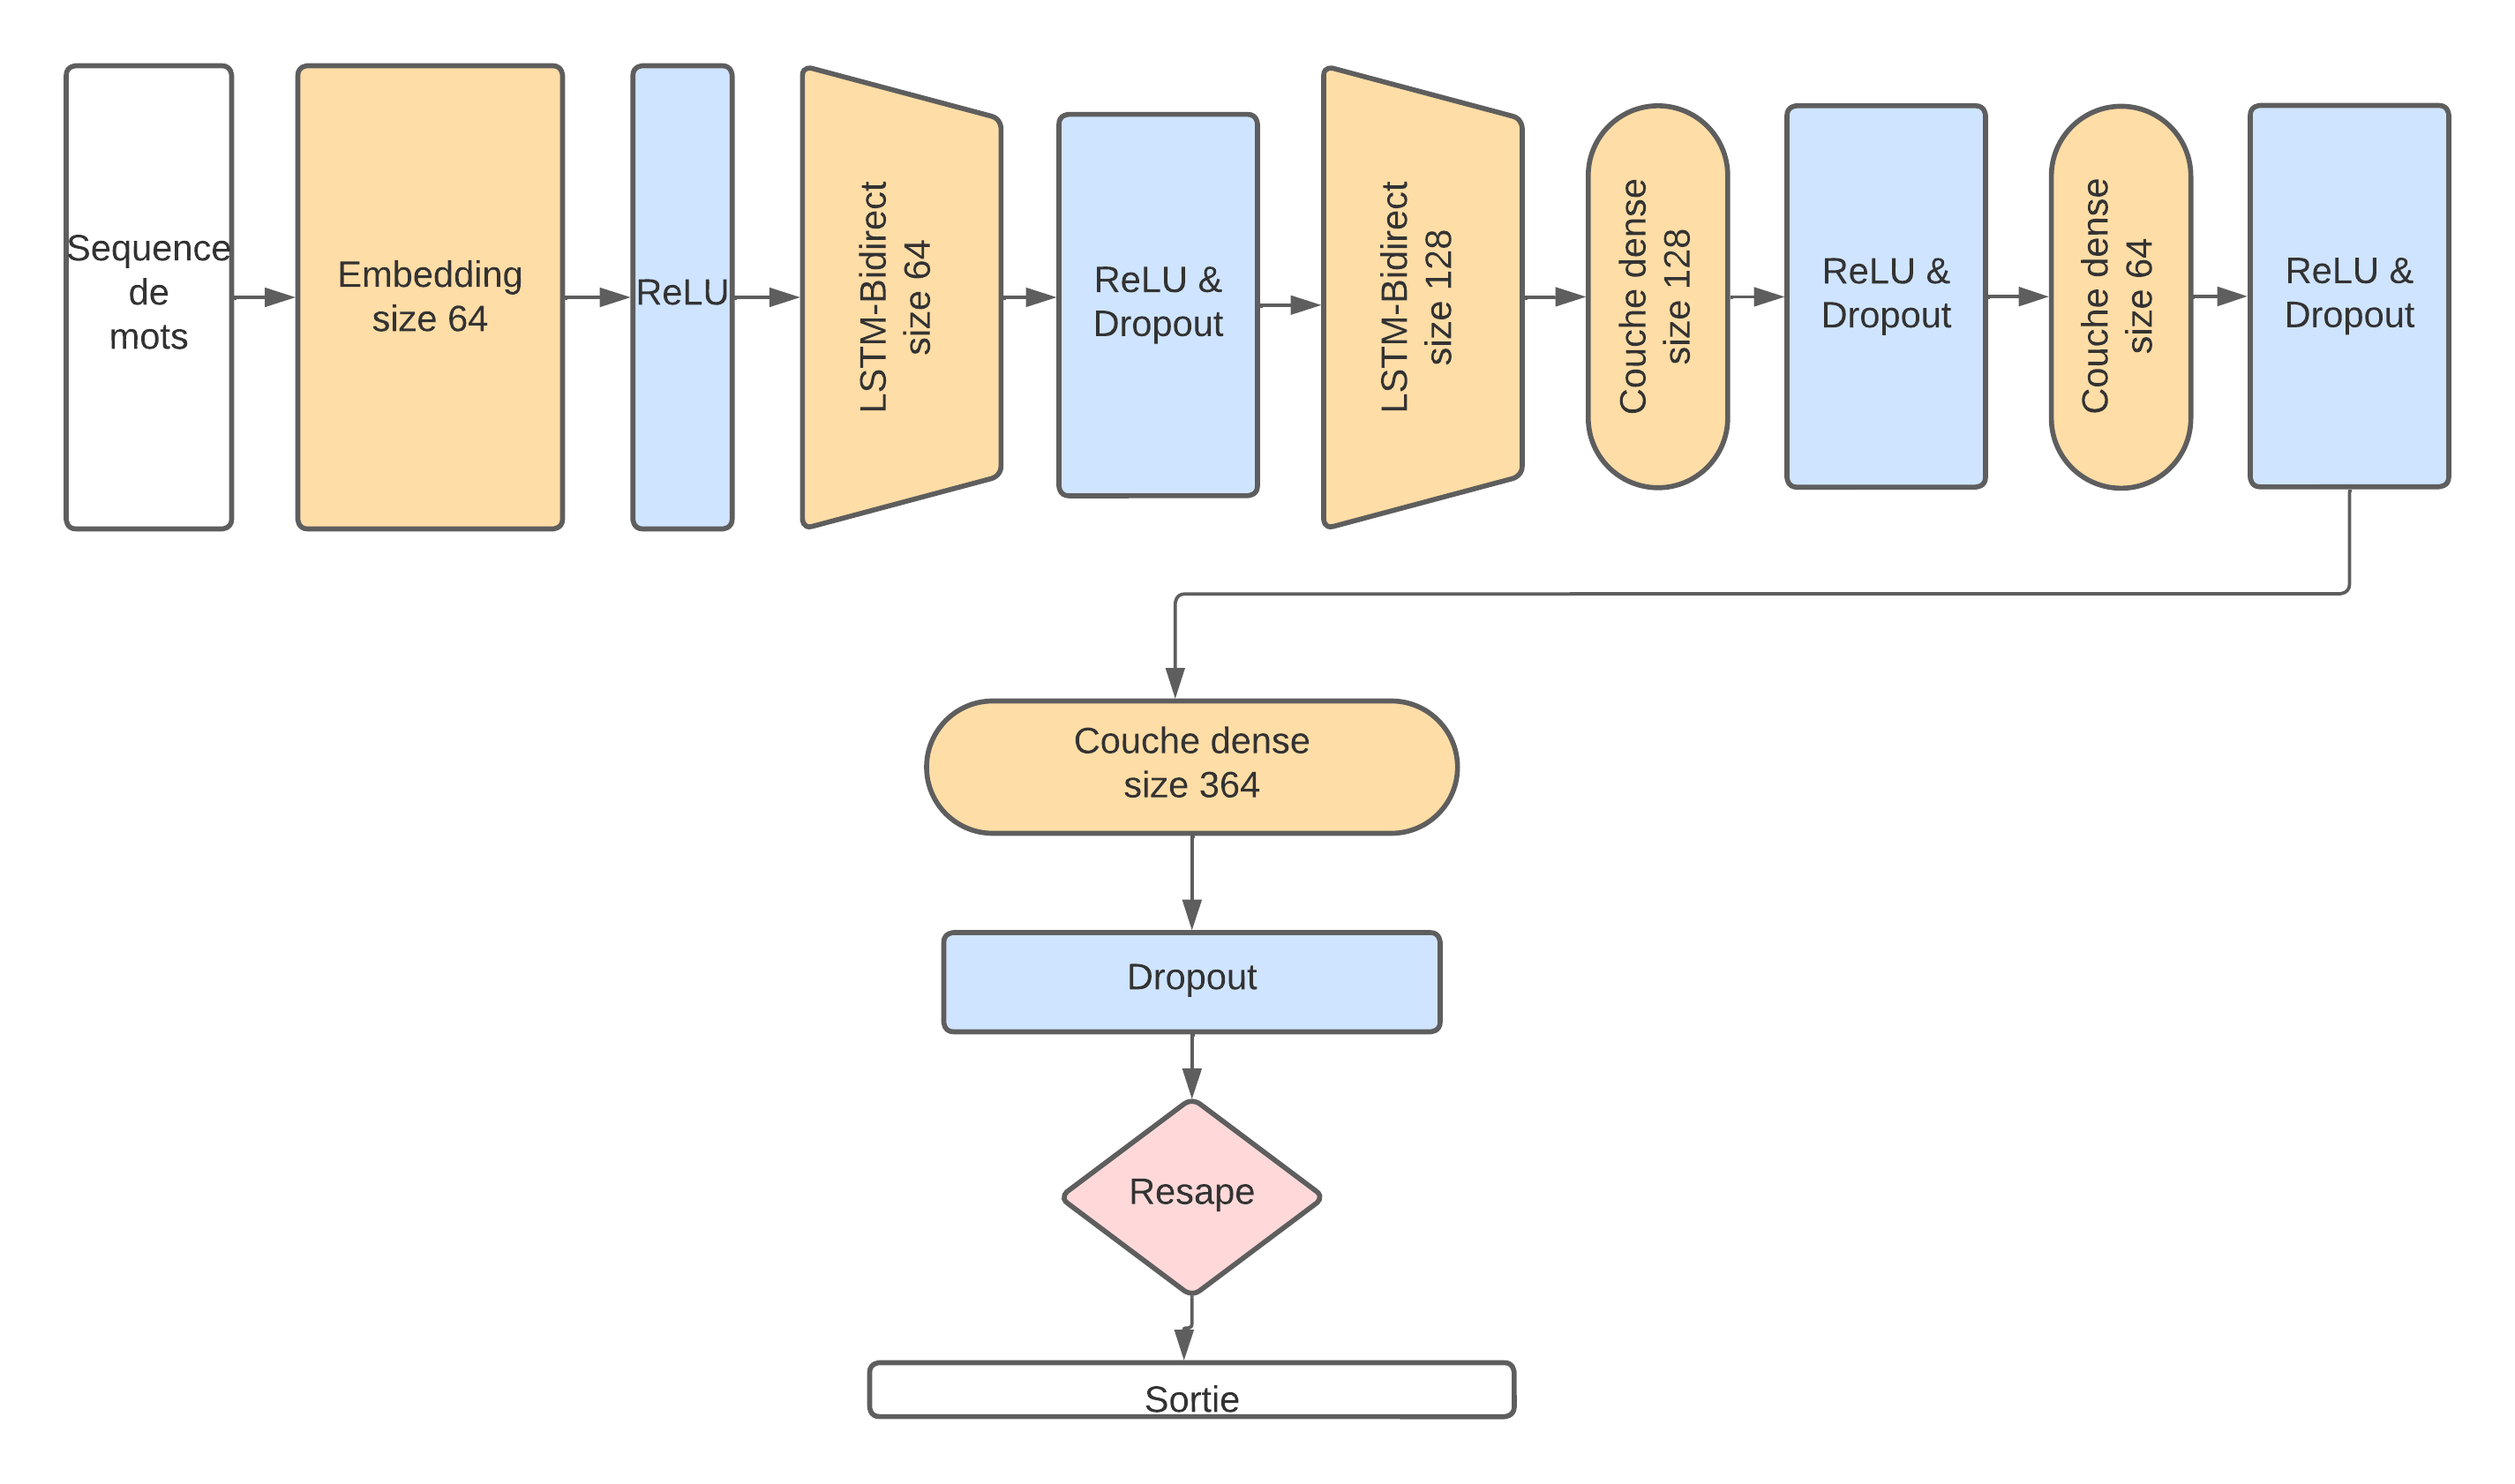
\includegraphics[width=\textwidth]{get_morphy_supertag.png}
        \caption{Modèle \textit{SUPERTAG}}
        \label{fig: model supertag}
    \end{figure}
\end{frame}

\begin{frame}{Modèle \textit{SEPARATE}}
    \begin{figure}
        \centering
        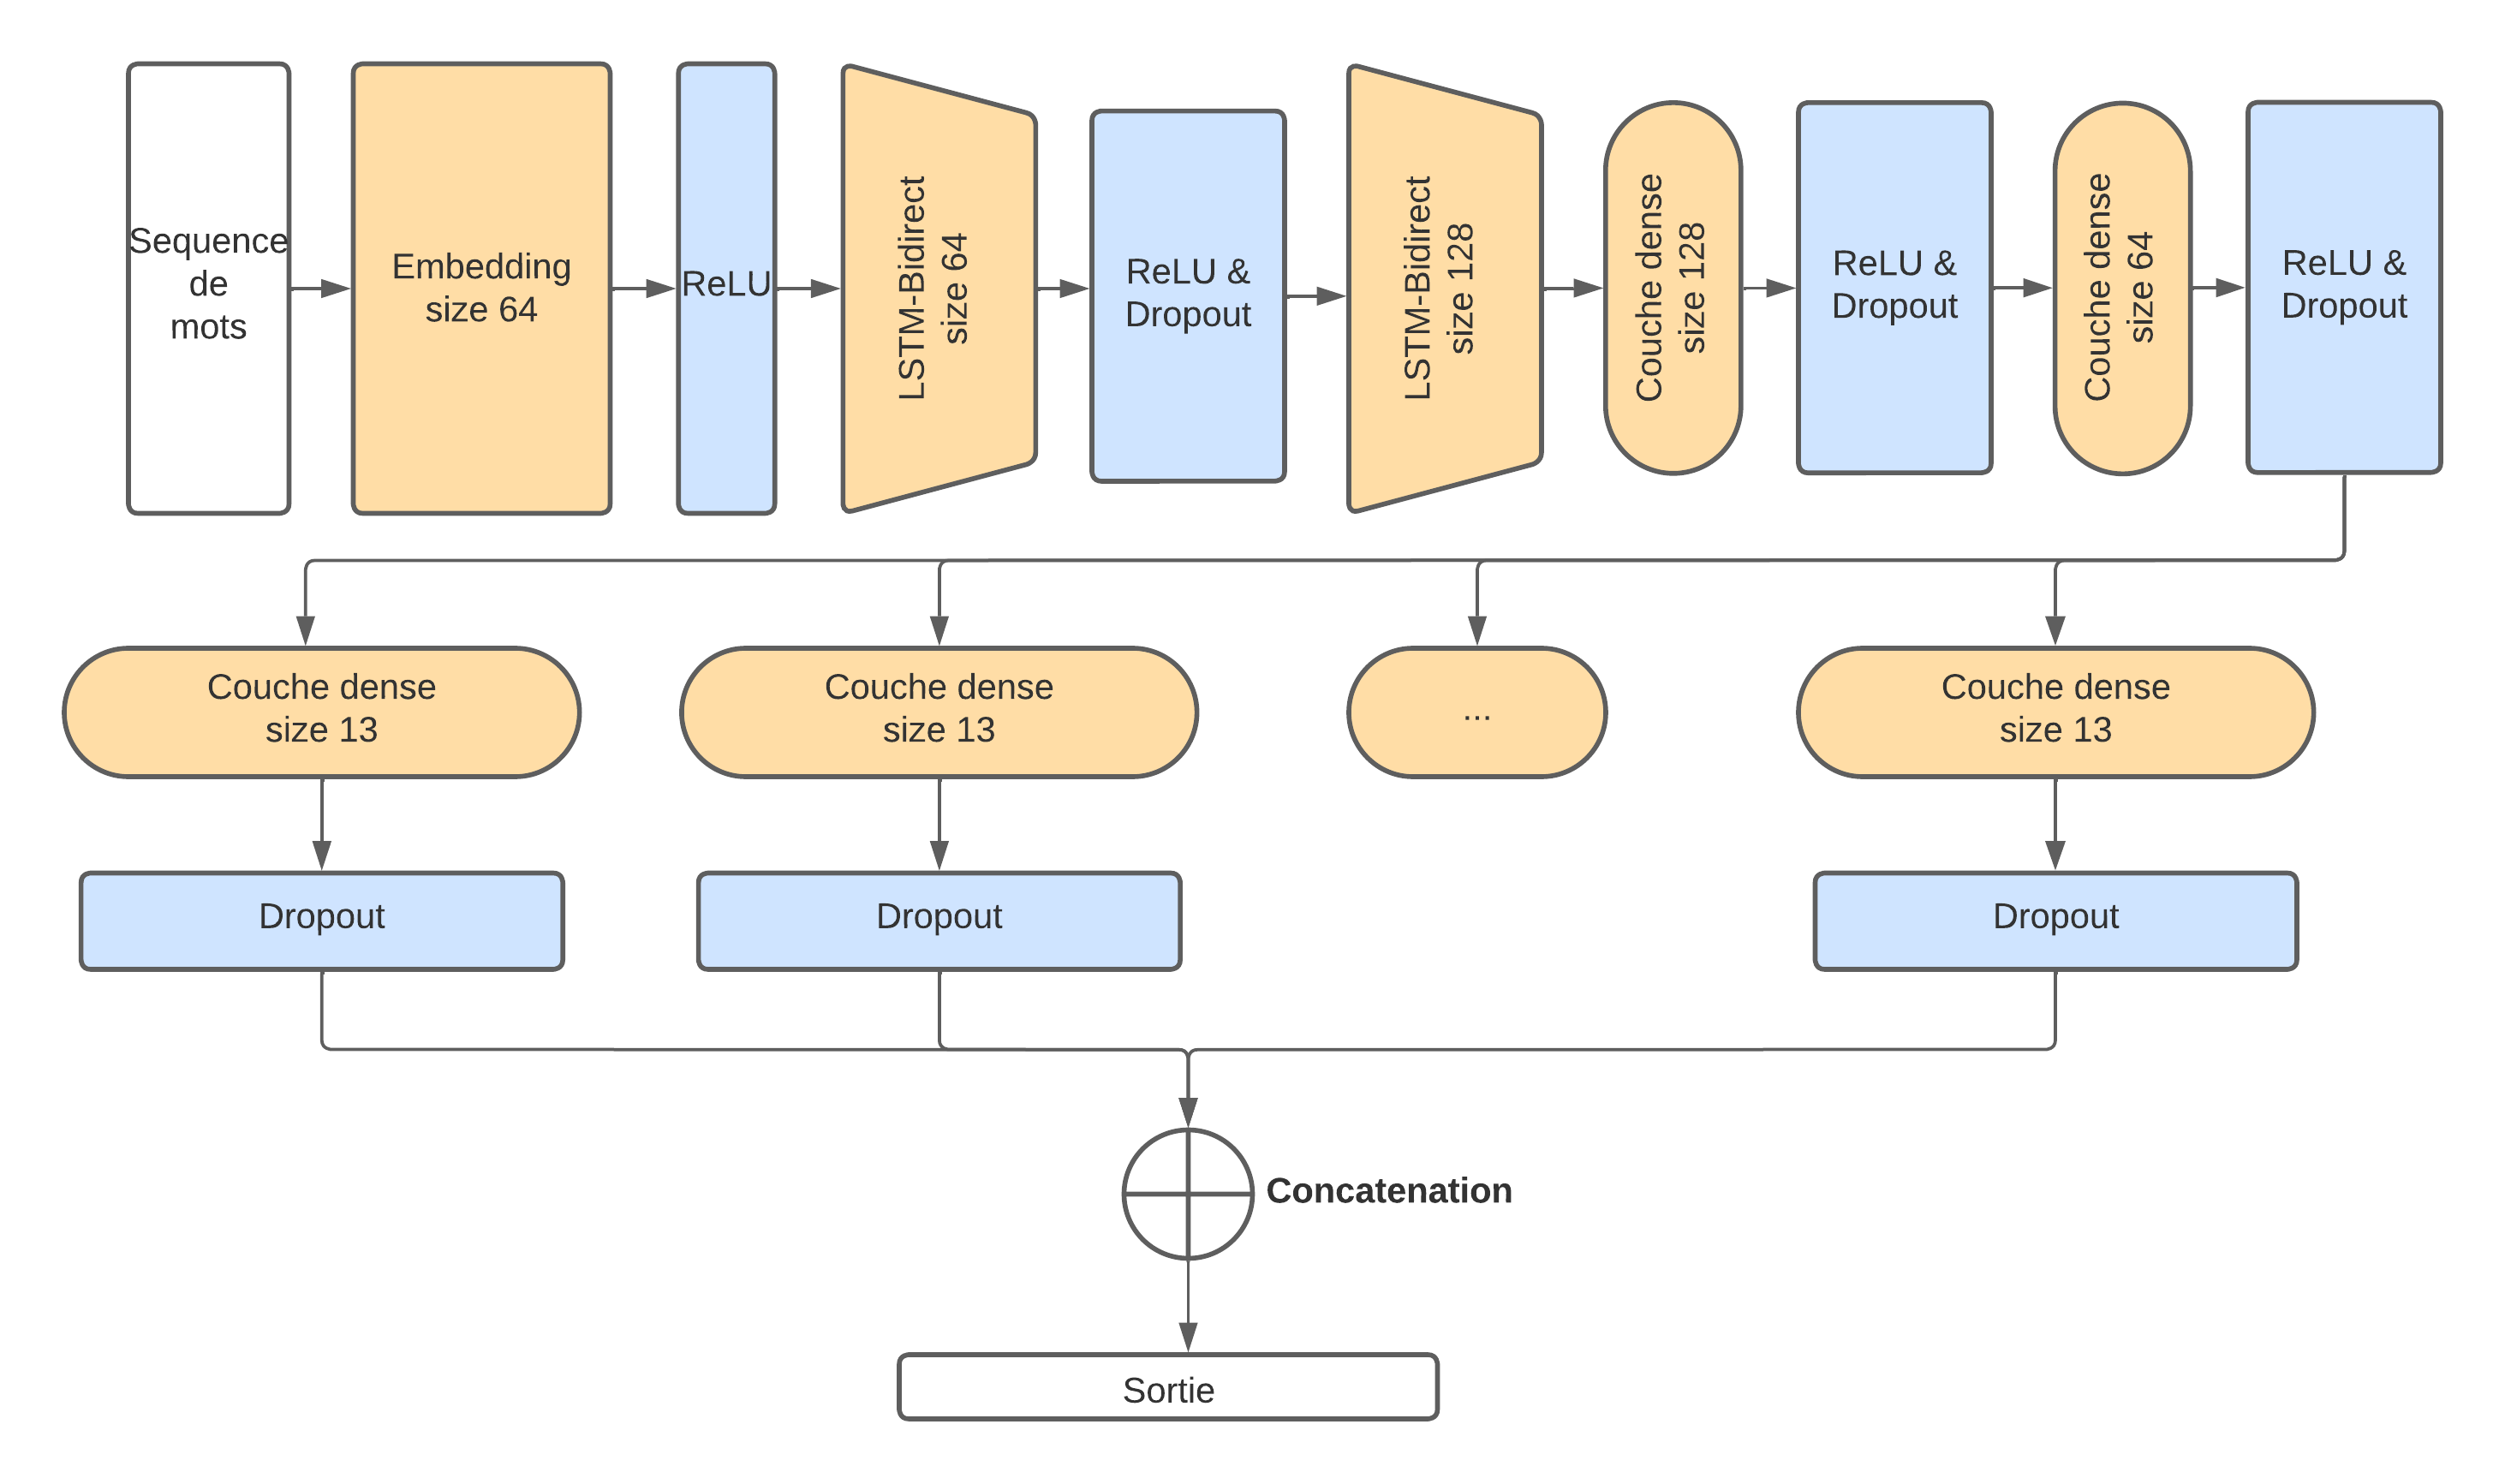
\includegraphics[width=\textwidth]{get_morphy_separate.png}
        \caption{Modèle \textit{SEPARATE}.}
        \label{fig: model separate}
    \end{figure}
\end{frame}

\begin{frame}{Modèle \textit{FUSION}}
    \begin{figure}[!ht]
        \centering
        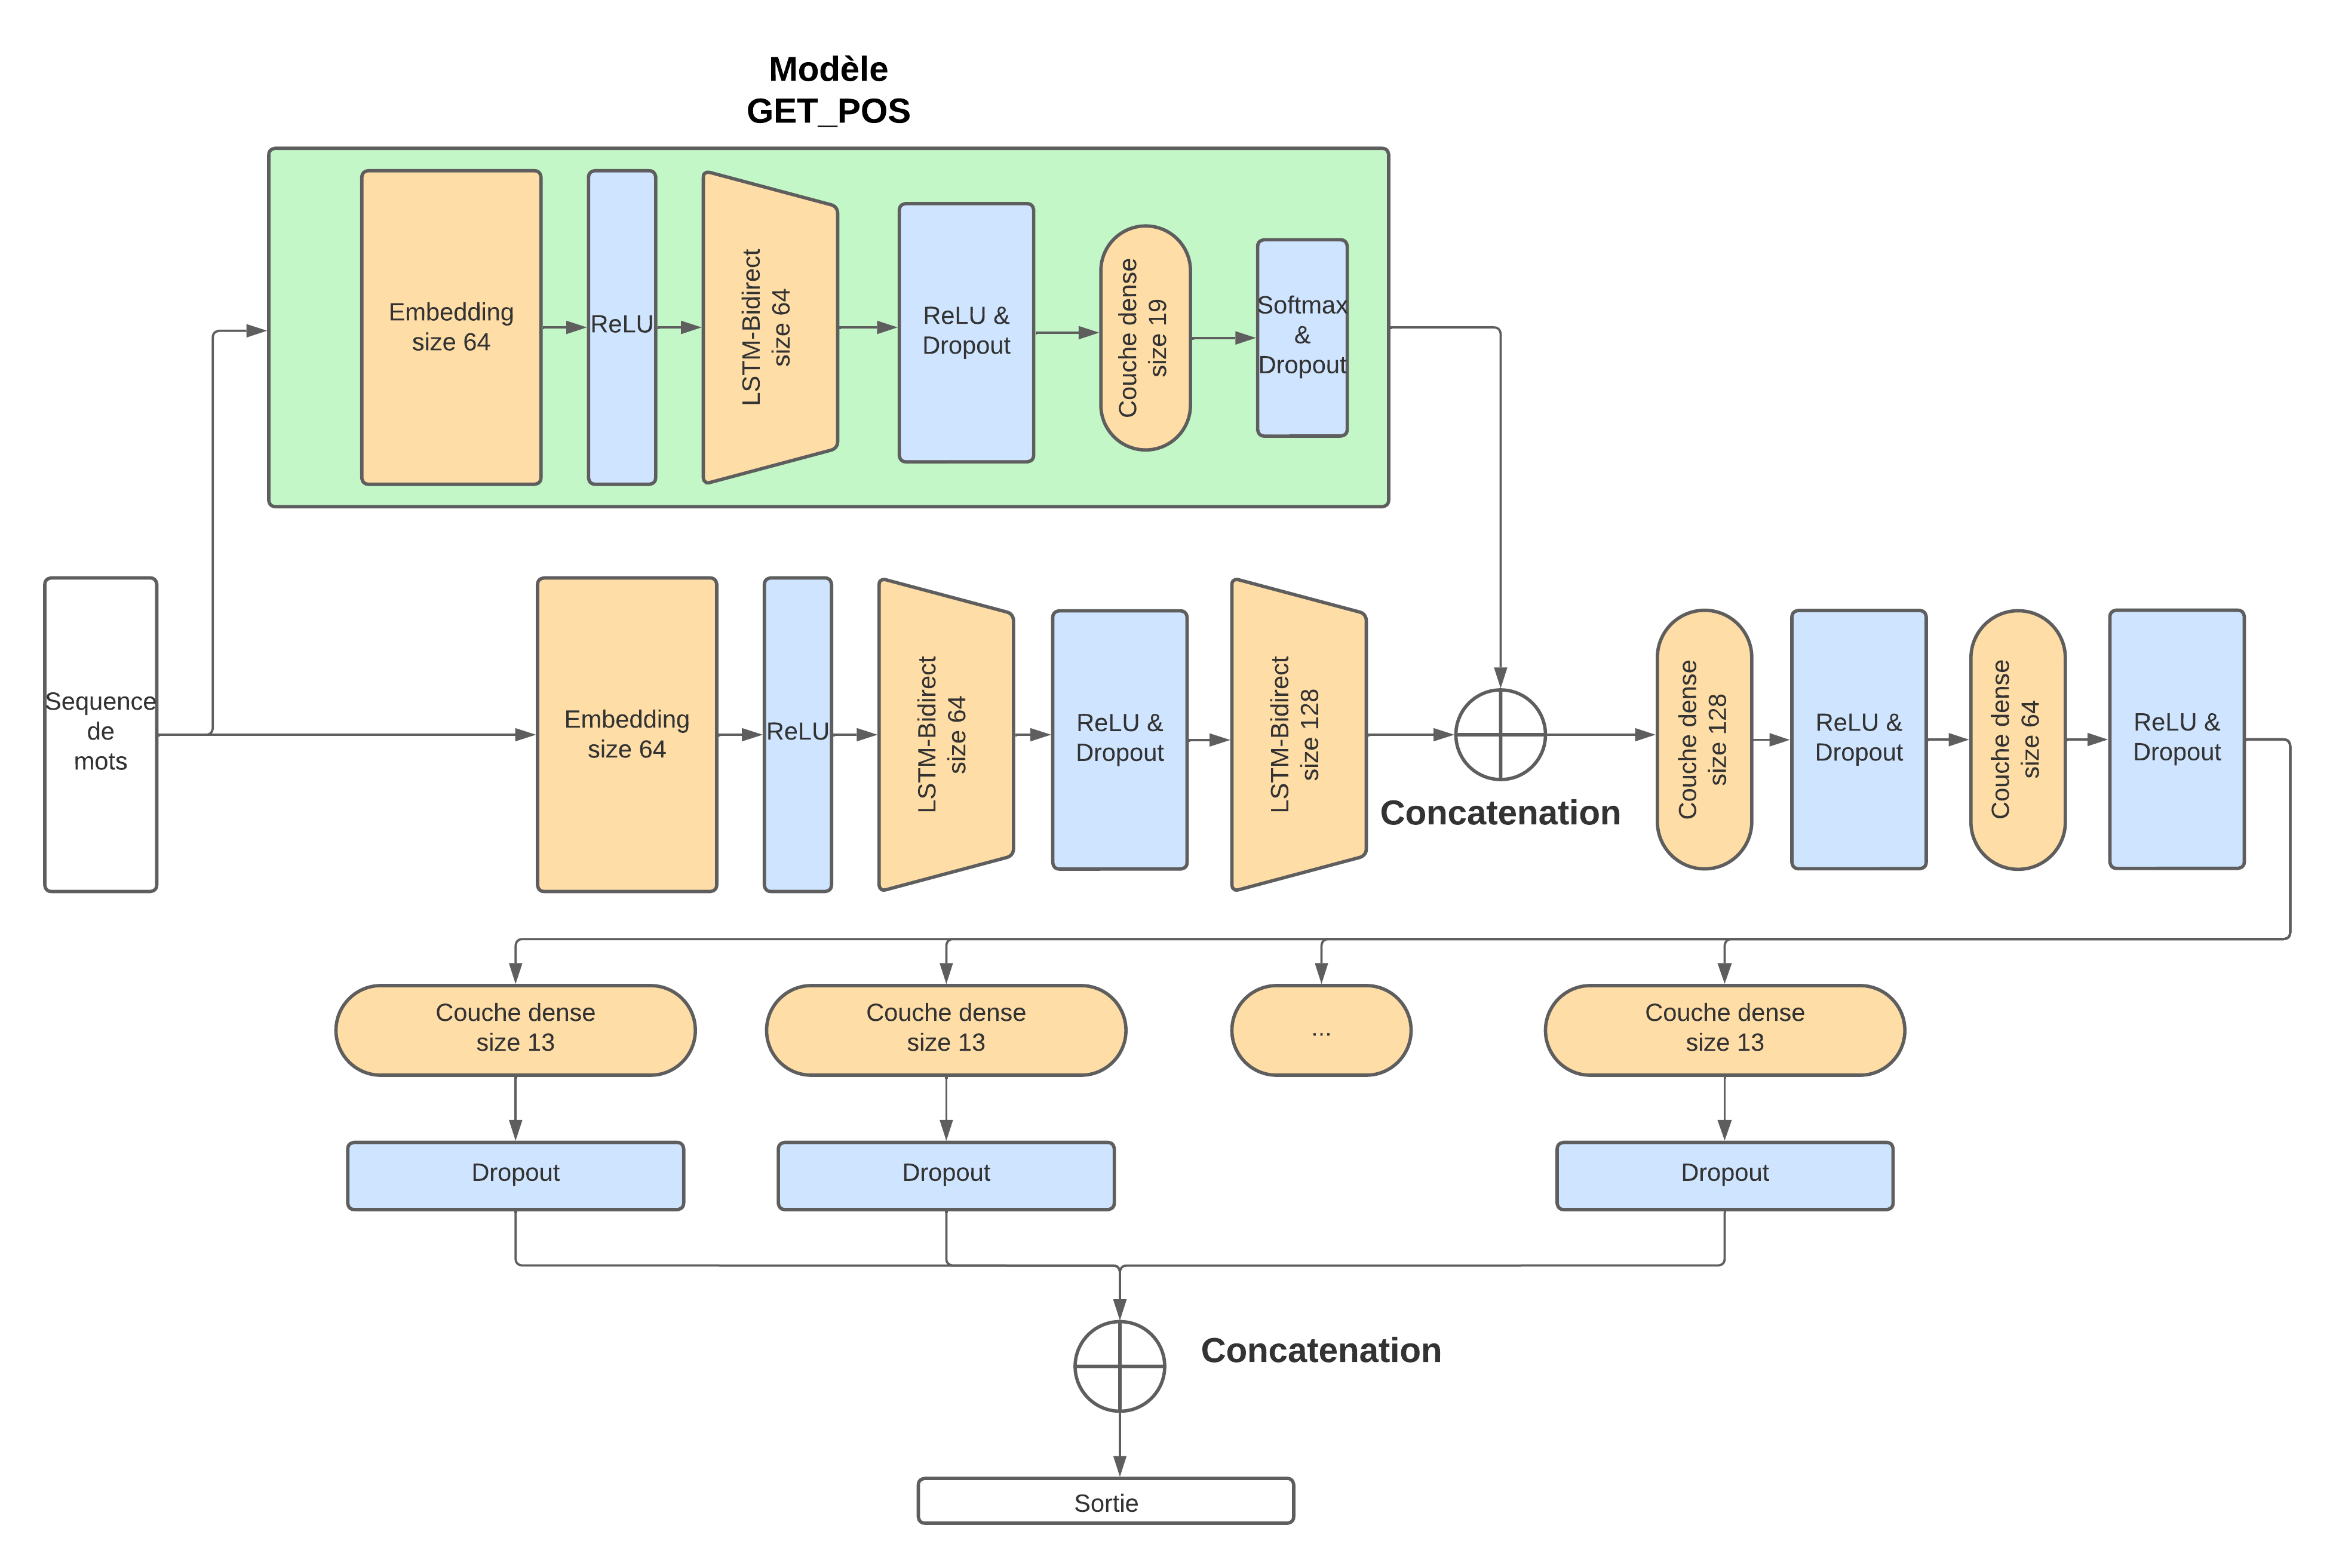
\includegraphics[width=\textwidth]{get_morphy_fusion.png}
        \caption{Modèle \textit{FUSION}}
        \label{fig: model fusion}
    \end{figure}
\end{frame}





\end{document}

